\documentclass[12pt]{article}

\usepackage{pgfplots}
\usepackage[margin=0.5in,paperwidth=6.2in,paperheight=3.7in]{geometry}

\begin{document}

\thispagestyle{empty}

\begin{figure}[h]
	\begin{center}
		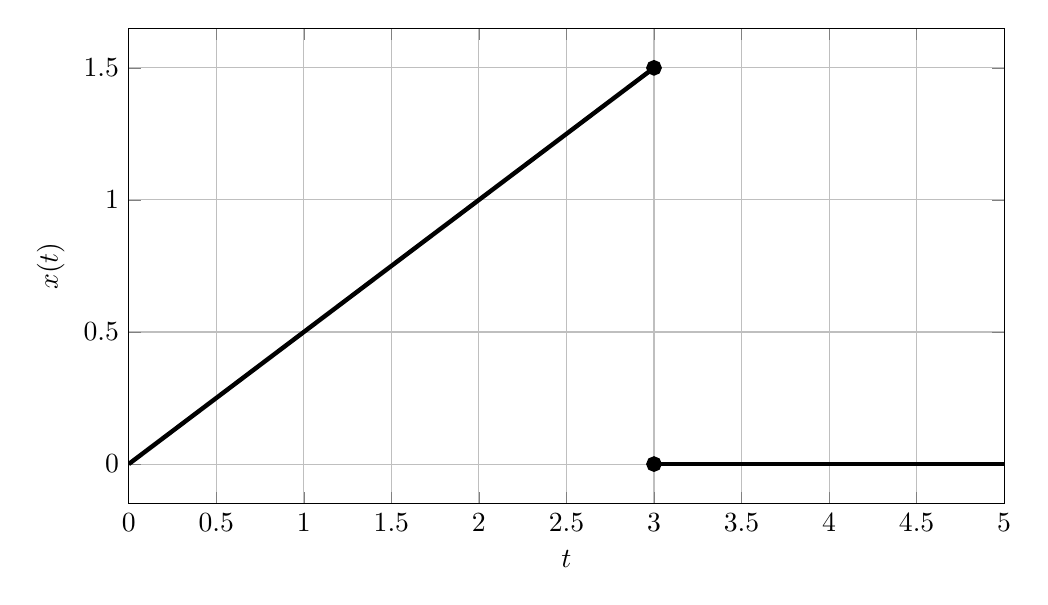
\begin{tikzpicture}
			\begin{axis}[
					width=5in,
					height=3in,
					grid=both,
					xmin=0, xmax=5,
					xlabel=$t$,
					ylabel=$x(t)$
				]
				\addplot[ultra thick, black, domain=0:3, samples=10]{0.5*x};
				\addplot[ultra thick, black, domain=3:5, samples=10]{0};
				\addplot[ultra thick, black, only marks] table {
						3 1.5
						3 0
					};
			\end{axis}
		\end{tikzpicture}
	\end{center}
\end{figure}

\end{document}
